\section{The finite cubical theorem}\label{sec:finite}

\subsection{Orientation and sampled expressions}

For $1\le i\le k$ and $\varepsilon\in\{0,1\}$, let
$\delta_i^\varepsilon:Q^{k-1}\to Q^k$ insert $\varepsilon$ as coordinate $i$,
leaving the other coordinates in increasing order. The standard orientation
is $\dd x_1\wedge\cdots\wedge\dd x_k$ and the oriented boundary is
\begin{equation}\label{eq:cube-boundary}
 \partial Q^k=\sum_{i=1}^k(-1)^{i-1}
       \bigl(\delta_i^1-\delta_i^0\bigr).
\end{equation}
Write a $(k-1)$-form in flux notation as
\begin{equation}\label{eq:flux-form}
 \omega=\sum_{i=1}^k(-1)^{i-1}f_i\,
  \dd x_1\wedge\cdots\wedge\widehat{\dd x_i}
                  \wedge\cdots\wedge\dd x_k .
\end{equation}
Moving $\dd x_i$ into position $i$ contributes another $(-1)^{i-1}$, so
\[
 \dd\omega=\Bigl(\sum_{i=1}^kg_i\Bigr)
                    \dd x_1\wedge\cdots\wedge\dd x_k,
 \qquad g_i=\partial_i f_i.
\]
On face $i$, every term of \eqref{eq:flux-form} except $f_i$ vanishes on
pullback. The sign of that term cancels the sign in
\eqref{eq:cube-boundary}. This explains why the finite formula below has
upper-minus-lower faces with no further signs.

Put $N=2^n$, $h=1/N$, and $x_a=ha$ for
$a\in\Grid{N}{k}$. Define exact rational expressions
\begin{align}
 V_{n,p}
  &=h^k\sum_{a\in\Grid{N}{k}}\sum_{i=1}^kG_i(x_a,p),
       \label{eq:V}\\
 B_{n,p}
  &=h^{k-1}\sum_{i=1}^k\sum_{b\in\Grid{N}{k-1}}
    \left(F_i(\delta_i^1(hb),p)-F_i(\delta_i^0(hb),p)\right),
       \label{eq:B}\\
 T_{n,p}
  &=h^{k-1}\sum_{a\in\Grid{N}{k}}\sum_{i=1}^k
       \left(F_i(x_a+he_i,p)-F_i(x_a,p)\right).
       \label{eq:T}
\end{align}
For $k=1$, the set $\Grid{N}{0}$ consists of its single empty tuple, and
$h^0=1$. Thus the boundary sum in that case is exactly $F_1(1,p)-F_1(0,p)$.
No exceptional analytic argument is needed for dimension one.

\begin{lemma}[Exact telescoping]\label{lem:telescoping}
For all sampled rational tables, independently of any continuity or
differentiability assumptions,
\[
 T_{n,p}=B_{n,p}.
\]
\end{lemma}
\begin{proof}
Fix $i$ and all coordinates other than coordinate $i$. Set
\[
 A(j)=F_i(x_1,\ldots,x_{i-1},jh,x_{i+1},\ldots,x_k,p).
\]
For every $m\le N$,
\begin{equation}\label{eq:prefix-telescope}
 \sum_{j<m}(A(j+1)-A(j))=A(m)-A(0).
\end{equation}
At $m=0$ both sides are zero. At the successor, add
$A(m+1)-A(m)$ and cancel $A(m)$; this proves the invariant by
quantifier-free induction. Take $m=N$, multiply by $h^{k-1}$, and sum over
the $N^{k-1}$ transverse tuples and the $k$ directions. Reordering these
finite sums is repeated finite distributivity, or finite Fubini. The result
is exactly \eqref{eq:B}.
\end{proof}

\begin{figure}[htbp]
\centering
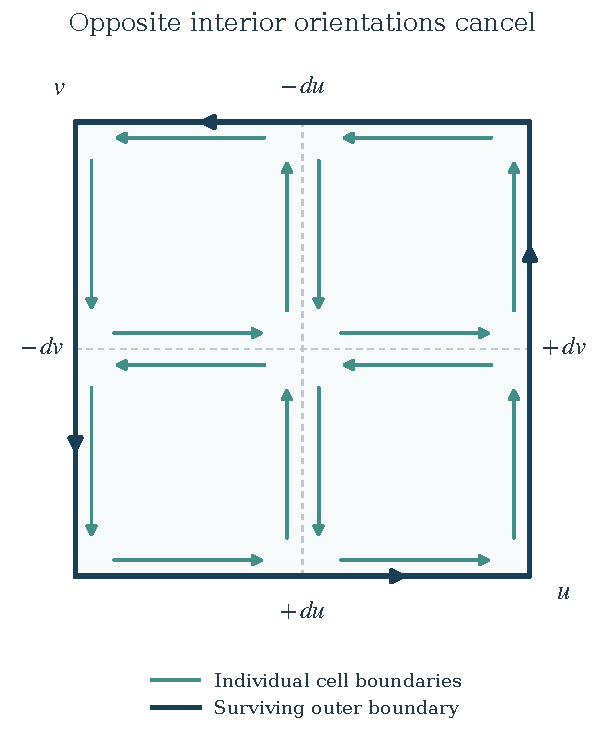
\includegraphics[width=0.52\textwidth]{figures/grid_cancellation.pdf}
\caption{The orientation mechanism in dimension two. Opposite
contributions on a shared grid edge cancel; the outside edges retain
the counterclockwise orientation. The finite telescope proves the
same cancellation in every fixed dimension.}
\label{fig:cancellation}
\end{figure}
\FloatBarrier

\begin{theorem}[Finite Stokes with evaluation errors]\label{thm:finite}
Assume the coordinate remainder certificate
\eqref{eq:derivative-cert}. If $n\ge\tau(t)$, then
\begin{equation}\label{eq:finite-bound}
 \boxed{\quad
 \abs{V_{n,p}-B_{n,p}}
 \le k\,2^{-t}+k(2N+1)2^{-p},\qquad N=2^n .
 \quad}
\end{equation}
\end{theorem}
\begin{proof}
Since $h\le2^{-\tau(t)}$ and each forward edge remains in $Q^k$,
\eqref{eq:derivative-cert} applies to every pair $(a,i)$. Write its residual
as
\[
 R_{a,i}=F_i(x_a+he_i,p)-F_i(x_a,p)-hG_i(x_a,p).
\]
It satisfies
$|R_{a,i}|\le h2^{-t}+(2+h)2^{-p}$.
By \cref{lem:telescoping},
\[
 B_{n,p}-V_{n,p}=h^{k-1}\sum_{a,i}R_{a,i}.
\]
There are precisely $kN^k$ summands. The finite triangle inequality therefore
gives
\begin{align*}
 \abs{B_{n,p}-V_{n,p}}
 &\le h^{k-1}kN^k
             \left(h2^{-t}+(2+h)2^{-p}\right)\\
 &=k2^{-t}+k(2N+1)2^{-p},
\end{align*}
because $N^kh^k=1$ and $N^kh^{k-1}=N$. This uses only finite rational
identities and inequalities.
\end{proof}

\begin{remark}[Why the precision must depend on the mesh]
Exact cancellation of identical samples does not remove the evaluation
term from the \emph{local remainder estimate}. Each comparison with a
derivative involves two coefficient evaluation errors. Summing their
absolute bounds produces $2kN2^{-p}$. Keeping $p$ fixed while increasing $N$
would make this bound worse. The schedule in the next section explicitly
increases $p$ with $n$. The analogous one-dimensional issue is already
identified in the inspected calculus packet \cite{repo-calculus}.
\end{remark}

\subsection{An optional sharper exact-evaluation version}

If the coefficient and derivative values are rational and are evaluated
exactly, and
\[
 \abs{f_i(x+he_i)-f_i(x)-hg_i(x)}\le C_i h^2,
\]
the same proof yields
\[
 \abs{V_N-B_N}\le h\sum_{i=1}^kC_i.
\]
This is useful for polynomial examples. It is not substituted for
\eqref{eq:finite-bound} in the general theorem, where values are available
only through approximation programs.

\FloatBarrier
\section{Constructing the integrals and proving equality}\label{sec:names-proof}

\subsection{A finite refinement lemma}

Let $H(x,p)$ satisfy (C) and (U) on $Q^d$, with modulus $\mu_H$.
Define its left-grid sum
\[
 R_H(n,p)=2^{-nd}\sum_{a\in\Grid{2^n}{d}}H(2^{-n}a,p).
\]
The definition includes $d=0$: the sum has one term and weight one.

\begin{lemma}[Dyadic refinement]\label{lem:refinement}
If $m\ge n\ge\mu_H(t)$, then
\begin{equation}\label{eq:refinement}
 \abs{R_H(n,p)-R_H(m,q)}
 \le2^{-t}+2^{-p}+2^{-q}.
\end{equation}
\end{lemma}
\begin{proof}
Let $L=2^{m-n}$. Every fine index has the unique coordinatewise decomposition
$b=La+c$, with $a\in\Grid{2^n}{d}$ and $c\in\Grid{L}{d}$.
Its fine sample is $2^{-m}b=2^{-n}a+2^{-m}c$. Its distance from the
coarse sample is at most $2^{-n}$, so (U) bounds the difference of the
two sampled values by the right side of \eqref{eq:refinement}.
For each $a$, there are $L^d$ fine points, and
$L^d2^{-md}=2^{-nd}$. Rewrite the coarse sum using those repeated fine
weights, subtract the fine sum, and apply the finite triangle inequality.
The sum of all weights is one. When $d=0$ the same calculation has one
point and uses the zero distance between that point and itself.
\end{proof}

This proof is a grouping identity for finite sums. It invokes neither a
measure-theoretic Fubini theorem nor convergence of an infinite sequence.

\subsection{An integral is an explicitly specified name}

For one coefficient define
\begin{equation}\label{eq:generic-integral-name}
 I_H(r)=R_H\bigl(\max\{r,\bar\mu_H(r+2)\},\,r+2\bigr).
\end{equation}
For $s\ge r$, \cref{lem:refinement} gives
\[
 \abs{I_H(r)-I_H(s)}
 \le 2^{-(r+2)}+2^{-(r+2)}+2^{-(s+2)}
 \le2^{-r}+2^{-s}.
\]
Thus $I_H$ is a primitive recursive regular name. We define
$\int_{Q^d}H$ to be its equality class in the shorthand of
\eqref{eq:name-equality}. The object theory needs only the name and the
formula, not an actual quotient sort.

Any other primitive recursive grid-and-evaluation schedule with an
explicit convergence rate represents the same integral, after
reindexing to a regular name when necessary, if its mesh
eventually satisfies the prescribed modulus and its evaluation precision
tends to infinity with a prescribed rate. Indeed, compare the two dyadic
grids at a target accuracy using \cref{lem:refinement}, taking the smaller
grid first, and then apply \cref{lem:slack}.

Finite linearity follows in the same way. At a common grid and sufficiently
guarded evaluation precision, addition and scalar multiplication are
identities of rational sums; the accumulated approximation error is
bounded by the sum of the coefficient weights. Refinement then proves
the equality of the associated names. In particular a sum of $M$ terms
requires at most an additional $\ell(M)$ precision bits, and an integer
linear combination uses $\ell(\max\{1,\sum|c_j|\})$.

\subsection{One schedule for both sides of Stokes}

Let $\ell=\ell(k)$. Define
\begin{align}
 t_r &= r+\ell+4,\label{eq:schedule-t}\\
 n_r &= \max\{r,\bar\mu_F(t_r),\bar\mu_G(t_r),\bar\tau(t_r)\},
       \label{eq:schedule-n}\\
 p_r &= n_r+t_r+2,\label{eq:schedule-p}\\
 V_r &= V_{n_r,p_r},\qquad B_r=B_{n_r,p_r}.\label{eq:schedule-values}
\end{align}
All functions in this display are primitive recursive. Both $n_r$ and
$p_r$ are nondecreasing. The factor $2^{n_r}$ may be large; the theorem is
about primitive recursive construction, not a polynomial-time algorithm.

\begin{theorem}[Explicit Cauchy and equality rates]\label{thm:rates}
Under (C), (U), and (D), for $s\ge r$,
\begin{align}
 \abs{V_r-B_r}&\le\frac7{64}\,2^{-r},\label{eq:rate-diagonal}\\
 \abs{V_r-V_s}&\le\frac3{32}\,2^{-r},\label{eq:rate-volume}\\
 \abs{B_r-B_s}&\le\frac3{16}\,2^{-r}.\label{eq:rate-boundary}
\end{align}
The functions $V,B$ are regular names, represent the volume and boundary
integrals in \eqref{eq:stokes-intro}, and satisfy $V\EqName B$.
\end{theorem}
\begin{proof}
Put $N=2^{n_r}$. Since $2N+1\le3N$ and
$2^{-p_r}=2^{-n_r}2^{-t_r}/4$, \cref{thm:finite} gives
\[
 \abs{V_r-B_r}
 \le \frac74\,k2^{-t_r}
 \le\frac7{64}\,2^{-r},
\]
where $k\le2^\ell$ was used in the last step.

For the volume sums, apply \cref{lem:refinement} to each $G_i$ and sum.
Since $p_s\ge p_r\ge t_r+2$,
\[
 \abs{V_r-V_s}
 \le k\left(2^{-t_r}+2^{-p_r}+2^{-p_s}\right)
 \le\frac32\,k2^{-t_r}
 \le\frac3{32}\,2^{-r}.
\]
For the boundary sums there are $2k$ restricted coefficient functions.
Face insertion preserves sup-norm distances, so the same modulus
$\mu_F$ applies to each of them. Their total bound is twice the preceding
bound, proving \eqref{eq:rate-boundary}.

These inequalities imply \eqref{eq:regular} after deciding whether $r\le s$
or $s\le r$. The schedules tend to finer meshes and higher precision
explicitly, so \cref{lem:refinement} and finite linearity identify their
names with the integrals defined in \eqref{eq:generic-integral-name}.

Finally let $a,b\ge r$. If $a\le b$, insert $B_a$:
\[
 \abs{V_a-B_b}
 \le\abs{V_a-B_a}+\abs{B_a-B_b}
 \le\left(\frac7{64}+\frac3{16}\right)2^{-a}
 \le\frac{19}{64}\,2^{-r}.
\]
If $b\le a$, insert $V_b$ and obtain the smaller constant
$3/32+7/64=13/64$. This proves \eqref{eq:headline}.
Taking $r=\min\{a,b\}$ also yields
$|V_a-B_b|\le2^{-a}+2^{-b}$ directly. Hence $V\EqName B$.
\end{proof}

\begin{corollary}[Arithmetic form of cubical Stokes]\label{cor:arith-stokes}
For every fixed tuple of primitive recursive evaluators and moduli,
$\ipra$ proves
\[
 \mathsf H(F,G,\mu_F,\mu_G,\tau)\ \longrightarrow\
 \bigl(\mathsf{Name}(V)\wedge\mathsf{Name}(B)\wedge V\EqName B\bigr),
\]
as well as the explicit rational inequalities
\eqref{eq:rate-diagonal}--\eqref{eq:rate-boundary}.
\end{corollary}

The final universal quantifiers range over precision indices and rational
codes. In \cref{sec:ipra-audit} we give the induction invariants and
denominator-clearing procedure that justify the asserted $\ipra$
derivability. No general transfer theorem from constructive analysis to
$\ipra$ is being invoked.

\subsection{Stability under finite perturbations}

If two volume integrands differ pointwise by at most $\eta$ on a unit
cube, their integrals differ by at most $\eta$, with the corresponding
evaluation tolerances added at the finite level. The proof is a weighted
finite triangle inequality, followed by the same named-integral argument.
For a boundary made of $2k$ unit faces the analogous bound is $2k\eta$.
These estimates permit independently certified coefficient approximations
and are also the mechanism by which equal face parameterizations yield
equal face integrals.
